%%%
% Plantilla de Memoria
% Modificación de una plantilla de Latex de Nicolas Diaz para adaptarla 
% al castellano y a las necesidades de escribir informática y matemática%
% Editada por: Mario Román
%
% License:
% CC BY-NC-SA 3.0 (http://creativecommons.org/licenses/by-nc-sa/3.0/)
%%%

%%%%%%%%%%%%%%%%%%%%%%%%%%%%%%%%%%%%%%%%%
% Thin Sectioned Essay
% LaTeX Template
% Version 1.0 (3/8/13)
%
% This template has been downloaded from:
% http://www.LaTeXTemplates.com
%
% Original Author:
% Nicolas Diaz (nsdiaz@uc.cl) with extensive modifications by:
% Vel (vel@latextemplates.com)
%
% License:
% CC BY-NC-SA 3.0 (http://creativecommons.org/licenses/by-nc-sa/3.0/)
%
%%%%%%%%%%%%%%%%%%%%%%%%%%%%%%%%%%%%%%%%%

%----------------------------------------------------------------------------------------
%	PAQUETES Y CONFIGURACIÓN DEL DOCUMENTO
%----------------------------------------------------------------------------------------

%%% Configuración del papel.
% microtype: Tipografía.
% mathpazo: Usa la fuente Palatino.
\documentclass[a4paper, 20pt]{article}
\usepackage[a4paper,margin=1in]{geometry}
\usepackage[protrusion=true,expansion=true]{microtype}
\usepackage{mathpazo}

% Indentación de párrafos para Palatino
\setlength{\parindent}{0pt}
  \parskip=8pt
\linespread{1.05} % Change line spacing here, Palatino benefits from a slight increase by default


%%% Castellano.
% noquoting: Permite uso de comillas no españolas.
% lcroman: Permite la enumeración con numerales romanos en minúscula.
% fontenc: Usa la fuente completa para que pueda copiarse correctamente del pdf.
\usepackage[spanish,es-noquoting,es-lcroman,es-tabla,,es-nodecimaldot]{babel}
\usepackage[utf8]{inputenc}
\usepackage{fontenc}
\selectlanguage{spanish}


%%% Gráficos
\usepackage{graphicx} % Required for including pictures
\usepackage{wrapfig} % Allows in-line images
\usepackage[usenames,dvipsnames]{color} % Coloring code
%\usepackage{subcaption}
\usepackage{subfig}
\graphicspath{{./fig/}}


%%% Matemáticas
\usepackage{amsmath}
\usepackage{physics} % para las derivadas parciales
\usepackage[Symbol]{upgreek} %pi

%%% Pseudocódigo

\usepackage[htt]{hyphenat}
\usepackage{algorithmicx}
\usepackage[ruled]{algorithm}
\usepackage{algpseudocode}

\newcommand{\alg}{\texttt{algorithmicx}}
\newcommand{\old}{\texttt{algorithmic}}
\newcommand{\euk}{Euclid}
\newcommand\ASTART{\bigskip\noindent\begin{minipage}[b]{0.5\linewidth}}
\newcommand\ACONTINUE{\end{minipage}\begin{minipage}[b]{0.5\linewidth}}
\newcommand\AENDSKIP{\end{minipage}\bigskip}
\newcommand\AEND{\end{minipage}}

%%% Código
\usepackage{listings}
\lstset{
  basicstyle=\ttfamily,
  columns=fullflexible,
  %frame=single,
  breaklines=true
}

%%% Tablas
\usepackage{tabularx}
\usepackage{float}
\usepackage{adjustbox}
\usepackage{booktabs}

% Enlaces y colores
\usepackage{hyperref}
\usepackage[dvipsnames]{xcolor}
\definecolor{webgreen}{rgb}{0,0.5,0}
\hypersetup{
  colorlinks=true,
  citecolor=RoyalBlue,
  urlcolor=RoyalBlue,
  linkcolor=RoyalBlue
}

%%% Bibliografía
\usepackage[backend=biber]{biblatex}
\DefineBibliographyStrings{spanish}{
  urlseen = {Accedido}
}
\addbibresource{citations.bib}


\newcommand{\training}{\textit{training }}
\newcommand{\test}{\textit{test }}

%%% Subsubsection con letras
\renewcommand{\thesubsubsection}{\thesubsection.\alph{subsubsection}}

%%% Itemize, enumitem
\usepackage{paralist}
\usepackage{enumitem}
%----------------------------------------------------------------------------------------
%	TÍTULO
%----------------------------------------------------------------------------------------
% Configuraciones para el título.
% El título no debe editarse aquí.
\renewcommand{\maketitle}{
  \begin{flushright} % Right align
  
  {\LARGE\@title} % Increase the font size of the title
  
  \vspace{50pt} % Some vertical space between the title and author name
  
  {\large\@author} % Author name
  \\\@date % Date
  \vspace{40pt} % Some vertical space between the author block and abstract
  \end{flushright}
}

%% Título
\title{\textbf{Título}\\ % Title
Subtítulo} % Subtitle

\author{\textsc{Autor1,\\Autor2} % Author
\\{\textit{Universidad de Granada}}} % Institution

\date{\today} % Date

%-----------------------------------------------------------------------------------------
%	DOCUMENTO
%-----------------------------------------------------------------------------------------

\begin{document}

%-----------------------------------------------------------------------------------------
%	TITLE PAGE
%-----------------------------------------------------------------------------------------

\begin{titlepage} % Suppresses displaying the page number on the title page and the subsequent page counts as page 1
	
	\raggedleft % Right align the title page
	
	\rule{1pt}{\textheight} % Vertical line
	\hspace{0.05\textwidth} % Whitespace between the vertical line and title page text
	\parbox[b]{0.8\textwidth}{ % Paragraph box for holding the title page text, adjust the width to move the title page left or right on the page
		
		{\Huge\bfseries Trabajo 3:\\[0.5\baselineskip] Programación\\[0.5\baselineskip]\large AJUSTE DE MODELOS LINEALES\\[2\baselineskip]} % Title
		{\large\textit{Curso 2019/2020}\\[0.5\baselineskip]Aprendizaje Automático\\[1.5\baselineskip] }% Subtitle or further description
		{\Large\textsc{Sofía Almeida Bruno}\\[0.5\baselineskip]sofialmeida@correo.ugr.es} % Author name, lower case for consistent small caps
		
		\vspace{0.4\textheight} % Whitespace between the title block and the publisher
		
		{\noindent \\[0.5\baselineskip] }\\[\baselineskip] % Publisher and logo
	}

\end{titlepage}

%% Resumen (Descomentar para usarlo)
%\renewcommand{\abstractname}{Resumen} % Uncomment to change the name of the abstract to something else
%\begin{abstract}
% Resumen aquí
%\end{abstract}

%% Palabras clave
%\hspace*{3,6mm}\textit{Keywords:} lorem , ipsum , dolor , sit amet , lectus % Keywords
%\vspace{30pt} % Some vertical space between the abstract and first section


%% Índice
{\parskip=2pt
  \tableofcontents
}
\pagebreak

\section{\textit{Optical Recognition of Handwritten Digits Data Set}}
%% 1. Comprender el problema a resolver. Identificar los elementos X, Y and f del problema.
\subsection{Problema a resolver}

%% I ¿Qué base de datos tenemos?
%% I ¿Qué representan las columnas? ¿Son numéricas o
%% categóricas?
%% I ¿Qué hay en la variable de clase?
%% I ¿Se trata de un problema de aprendizaje supervisado o no
%% supervisado?
%% I ¿Es un problema de regresión o de clasificación?
El primer conjunto con el que vamos a trabajar es {\textit{Optical Recognition of Handwritten Digits Data Set}, reconocimiento óptico de dígitos escritos a mano \cite{opt_uci}. El código utilizado para trabajar con este conjunto de datos se encuentra en \texttt{optdigits.py}.

Se usaron programas del NIST (\textit{National Institute of Standards and Technology}) para extraer mapas de bits normalizados de dígitos escritos a mano. Un total de 43 personas contribuyeron a completar la base de datos; 30 personas añadiendo los números correspondientes al subconjunto de \training y 13 personas distintas incorporando los datos  de \test. Los mapas de bits originales son de tamaño $32\times 32$, pero se transforman en bloques no superpuestos de tamaño $4\times 4$ y se cuenta el número de píxeles de cada bloque, lo que nos dará una matriz de tamaño $8\times 8$ donde cada elemento es un entero en el intervalo $[0,16]$. Por tanto, de cada ejemplo tendremos 64 atributos, $n=64$, (uno por cada elemento de la matriz) y la variable objetivo. Como la variable objetivo, a pesar de ser numérica, representa el número que se ha escrito, consideraremos que estamos en un problema de clasificación en el que tenemos 10 clases (los números desde el 0 hasta el 9). Nos enfrentamos, por tanto, a un problema de clasificación multiclase. Además, el conjunto no presenta valores perdidos para ninguna variable.

En la Figura \ref{fig:digs} se han representado los primeros 20 ejemplos del conjunto de entrenamiento, considerando los datos como matrices $8\times 8$.

\begin{figure}[H]
    \centering
    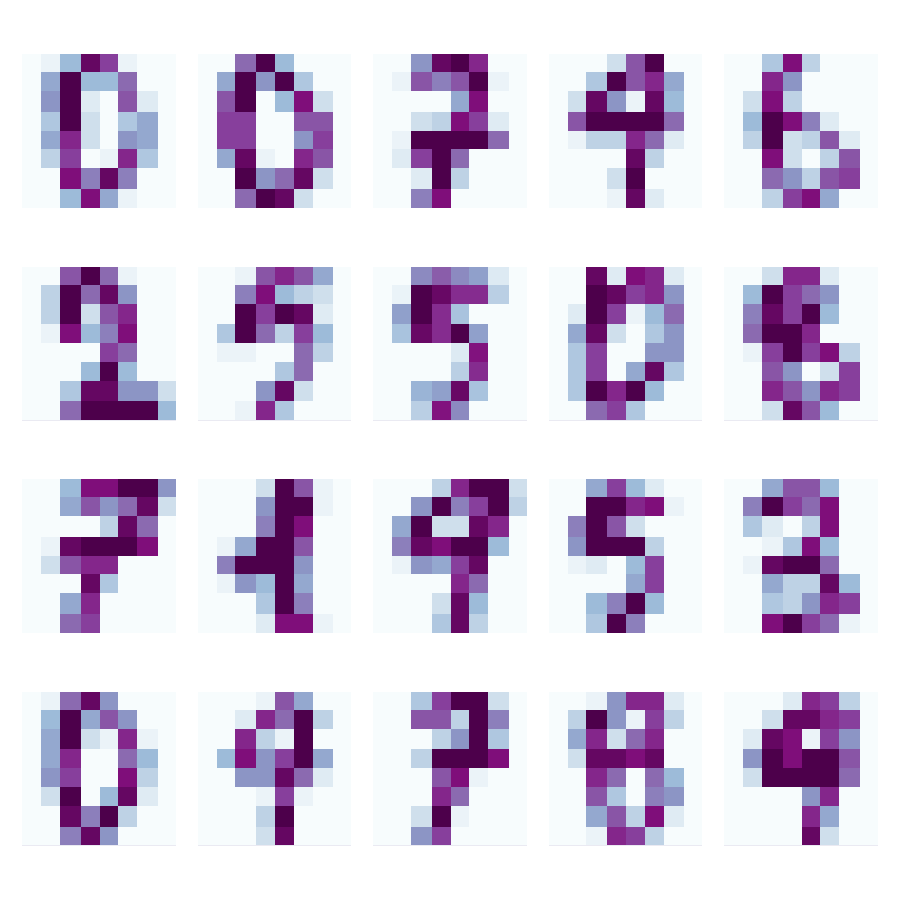
\includegraphics[width=0.75\textwidth]{Digits}
    \caption{Visualización de los primeros ejemplos del conjunto.}
    \label{fig:digs}
\end{figure}

Observamos la distribución de las clases del conjunto de entrenamiento en la Figura \ref{fig:histdigs}. La distribución es prácticamente uniforme con una diferencia máxima de elementos entre clases de 13 elementos. En conjunto formado por 3823 elementos esta diferencia es poco significativa, por lo que podemos afirmar que las clases de este conjunto están balanceadas.

\begin{figure}[H]
    \centering
    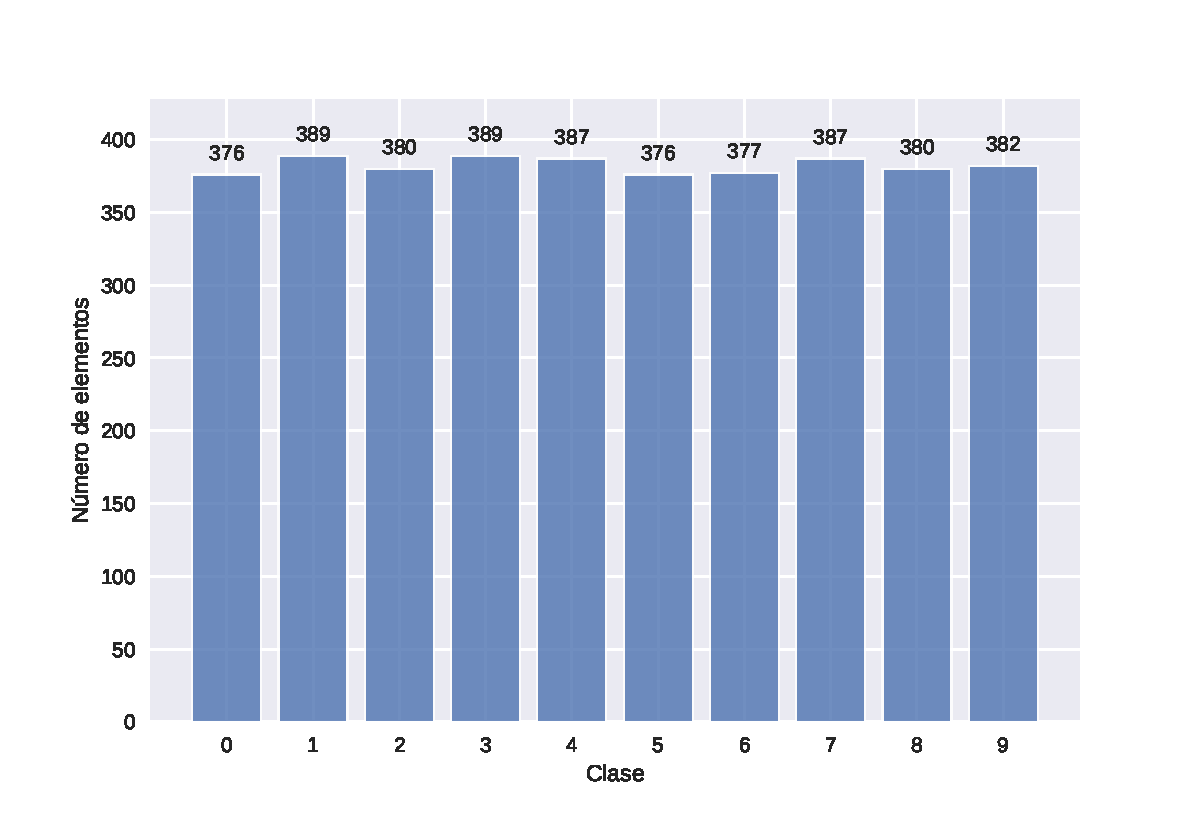
\includegraphics[width=1\textwidth]{HistDigits}
    \caption{Distribución de las clases en el conjunto de entrenamiento.}
    \label{fig:histdigs}
\end{figure}

%%%%%%%%%%%%%%%%%%%%%%%%%%%%%%%%%%%%%%%%%%%%%%%%%%%%%%%%%%%%%%%%%%%%%%%%
%% 2. Selección de las clase/s de funciones a usar. Identificar cuáles y porqué.
%%%%%%%%%%%%%%%%%%%%%%%%%%%%%%%%%%%%%%%%%%%%%%%%%%%%%%%%%%%%%%%%%%%%%%%%
\subsection{Clases de funciones}
% Combinaciones lineales, cuadráticas, etc... de las observaciones.
% Justificar su uso o por qué no se consideran necesarias.

Para realizar el aprendizaje se podría considerar la clase de funciones lineales en el vector de pesos $w$ que toma como hipótesis, $h\in \mathcal{H}$, funciones de la forma $h(x) = w^Tx$. Sin embargo, preferimos añadir complejidad a esta clase de funciones, utilizando una clase que, manteniendo la linealidad en $w$, no la mantenga para los vectores $x$. Esta será la de los polinomios hasta orden 2 de las variables. Analíticamente, \[
\mathcal{H} = \left \{ h(x) = w_{00} +\sum_{j=1}^nw_{0j}x_j + \sum_{i,j = 1}^nw_{ij} x_ix_j: w_{kj} \in \mathbb{R} \text{ para } k = 0,\cdots, n; j=0,\cdots,n\right\}.
\]
A priori no conocemos las relaciones entre las variables y no sabemos si serán lineales o no, añadir complejidad a la clase de funciones hace que, sin perder las posibilidades que tendríamos al no hacerlo, tengamos opciones de descubrir otro tipo de relaciones.

%%%%%%%%%%%%%%%%%%%%%%%%%%%%%%%%%%%%%%%%%%%%%%%%%%%%%%%%%%%%%%%%%%%%%%%
%% 3. Fijar conjuntos de training y test que sean coherentes.
%%%%%%%%%%%%%%%%%%%%%%%%%%%%%%%%%%%%%%%%%%%%%%%%%%%%%%%%%%%%%%%%%%%%%%
\subsection{Conjuntos de \textit{training} y \textit{test}}
%% TRAINING → Subconjunto de los datos que se estudia, se
%% visualiza y a la que se le aplican los modelos.
%% VALIDACIÓN → Subconjunto de los datos que indica cuál es el
%% mejor modelo.
%% TEST → Subconjunto de los datos que proporciona el error
%% cometido.
%% Posibles particiones:
%% I Si se decide usar el conjunto Validación: 50% training, 25%
%% Validación y 25% test.
%% I Si no se decide usar el conjunto de Validación: 70%
%% training y 30% test u 80% training y 20% test.

En este conjunto de datos los conjuntos de \training y \test ya vienen separados. Están formados por números escritos por grupos de personas diferentes. De esta forma, la información utilizada para entrenar el modelo y para realizar el \test será independiente.

El conjunto de \training está formado por 3823 ejemplos, $N_{\training} = 3823$, mientras que el de \test contiene 1797 ejemplos, $N_{\test} = 1797$. En total el conjunto tiene 5620 elementos, de los cuales se utiliza el 32\% para \test y el 68\% restante para entrenar el modelo, aproximadamente.

Además, para realizar el entrenamiento se realizará validación cruzada, utilizando 5 particiones, para tratar de evitar el sobreajuste que se puede producir por haber añadido complejidad a la clase de funciones.

%%%%%%%%%%%%%%%%%%%%%%%%%%%%%%%%%%%%%%%%%%%%%%%%%%%%%%%%%%%%%%%%%%%%%%%%
%% 4. Preprocesado los datos: codificación, normalización, proyección, etc. Es decir, todas las
%% manipulaciones sobre los datos iniciales hasta fijar el conjunto de vectores de caraterísticas
%% que se usarán en el entrenamiento.
%%%%%%%%%%%%%%%%%%%%%%%%%%%%%%%%%%%%%%%%%%%%%%%%%%%%%%%%%%%%%%%%%%%%%%%%
\subsection{Preprocesado}
%% ¿Por qué se preprocesan los datos?
%% Para eliminar impurezas y reducir la probabilidad de aprender de
%% manera errónea de los datos. Causas:
%% I Datos incompletos (Valores perdidos)
%% I Datos con ruido
%% I Datos inconsistentes

%% Tareas:
%% (esta lista es una sugerencia, por favor, elegid las que consideréis interesantes y/o necesarias)
%% I Colección, integración y transformación
%% Obtención de los datos, de una o más fuentes
%% Decodificación
%% Integración de datos de distintas bases de datos
%% Generación nuevo conocimiento
%% I Limpieza
%% - Modificación de datos con conflicto
%% - Eliminación de outliers
%% - Tratamiento de valores perdidos y problemas de ruido
%% I Reducción
%% - Selección de características
%% - Selección de instancias
%% - Discretización

El preprocesado está formado por dos tareas. La primera consiste en escalar los datos. Los datos originales se encontraban en el rango $[0,16]$, sin embargo, no sabemos si al añadir complejidad a la clase de funciones las nuevas variables a considerar se mantienen en ese rango (probablemente no, pues estamos haciendo productos de unas variables por otras). Los modelos de aprendizaje se implementan utilizando métodos numéricos, que en muchos casos funcionan mejor cuando los datos son cercanos a cero. Además, en la documentación de la técnica de ajuste a utilizar se indica que converge mejor cuando los datos están en la misma escala. Es por ello que se escalarán los datos de forma que tengan media 0 y desviación típica 1 \cite{scaler}.

Tras aumentar la complejidad de la clase de funciones pasamos de 64 variables a 2145. Son demasiadas, el tiempo de cómputo podría aumentar considerablemente. Además, no todas podrían resultar útiles para el aprendizaje, por ello, se realizará una selección de variables mediante regularización LASSO, que hemos visto en teoría que puede resultar útil como técnica de selección, al incentivar que el peso de algunas variables sea 0  \cite{lasso}. Tras realizar la selección tenemos 657 variables que son las que utilizaremos para realizar el aprendizaje.

%%%%%%%%%%%%%%%%%%%%%%%%%%%%%%%%%%%%%%%%%%%%%%%%%%%%%%%%%%%%%%%%%%%%%%%%
%% 5. Fijar la métrica de error a usar. Discutir su idoneidad para el problema.
%%%%%%%%%%%%%%%%%%%%%%%%%%%%%%%%%%%%%%%%%%%%%%%%%%%%%%%%%%%%%%%%%%%%%%%%
\subsection{Métrica de error}
%% Elegir la métrica a usar y discutir su elección. Teniendo en cuenta
%% si se trata de un problema de regresión o de clasificación, así
%% como el tipo de problema a tratar.
%% I Regresión Aquí y Aquí
%% I Clasificación Aquí

Nos encontramos en un problema de clasificación multiclase, es por esto, que la métrica elegida para evaluar la bondad de los modelos es el \textit{accuracy} \cite{acc}. Esta nos dará una media del número de aciertos. Si el vector de etiquetas reales de $N$ ejemplos es $y$ y el de las clases predichas es $y^{pred}$, el \textit{accuracy} será\[
accuracy(y, y^{pred}) = \frac{1}{N}\sum_{i=1}^N\mathbb{1}(y_i - y_i^{pred}),
\]
donde $\mathbb{1}$ es la función característica. Notamos que el \textit{accuracy} toma valores en el intervalo $[0,1]$, donde 1 es el máximo de aciertos, es decir, buscamos maximizarlo. Si queremos evaluar el error, consideraremos $1-accuracy$.

%%%%%%%%%%%%%%%%%%%%%%%%%%%%%%%%%%%%%%%%%%%%%%%%%%%%%%%%%%%%%%%%%%%%%%%%
%% 8. Identificar los modelos a usar.
%%%%%%%%%%%%%%%%%%%%%%%%%%%%%%%%%%%%%%%%%%%%%%%%%%%%%%%%%%%%%%%%%%%%%%%%
\subsection{Modelos}
%% Posibles modelos a usar:
%% I Regresión lineal
%% I Regresión logística
%% I Perceptrón + Pocket
Buscamos un modelo que nos permita clasificar las 10 clases. De los modelos vistos, el perceptrón queda descartado por ser específico de clasificación binaria. Tenemos que elegir entonces entre regresión logística y regresión lineal que, a pesar de tener nombres parecidos, son propios de diferentes tipos de problemas. Regresión logística es un modelo de clasificación binaria que, mediante \textit{SoftMax}, podemos adaptar para realizar una clasificación multiclase. Regresión lineal es una opción a considerar en este caso ya que las clases son numéricas, sin embargo, se descarta porque usando este método estaríamos asumiendo que las clases están ordenadas cuando, como clases o etiquetas, no lo están.

Por todos estos motivos, el modelo elegido es regresión logística.

%%%%%%%%%%%%%%%%%%%%%%%%%%%%%%%%%%%%%%%%%%%%%%%%%%%%%%%%%%%%%%%%%%%%%%%%
%% 6. Discutir la técnica de ajuste elegida.
%%%%%%%%%%%%%%%%%%%%%%%%%%%%%%%%%%%%%%%%%%%%%%%%%%%%%%%%%%%%%%%%%%%%%%%%
\subsection{Técnica de ajuste}
%% Según modelo a usar, qué técnica de ajuste utilizas (SGD,
%% Pseudoinversa...) y razone por qué lo has elegido.
La implementación de regresión logística a utilizar \cite{lreg} permite utilizar las siguientes técnicas: \texttt{‘liblinear’}, \texttt{‘lbfgs’}, \texttt{‘newton-cg’}, \texttt{‘sag’} y \texttt{‘saga’}. El primero de ellos se descarta pues no es una implementación de un problema multiclase real, utilizando la distribución multinomial para extender el caso binario en el que se utilizaba la distribución binomial. \texttt{lbfgs} se descarta pues en la documentación se indica que no es el que tiene el mejor rendimiento. Tanto \texttt{sag} como \texttt{saga}\footnote{Estas técnicas solo garantizan la convergencia cuando las características tengan aproximadamente la misma escala.} utilizan variantes del gradiente descendente estocástico y en la tabla comparativa se sugiere que son los más rápidos en conjuntos de datos grandes (como puede ser el nuestro tras aumentar el número de variables). Finalmente, se opta por elegir \texttt{saga} como técnica de ajuste por ser una versión posterior que trata de disminuir la velocidad.


%%%%%%%%%%%%%%%%%%%%%%%%%%%%%%%%%%%%%%%%%%%%%%%%%%%%%%%%%%%%%%%%%%%%%%
%% 7. Discutir la necesidad de regularización y en su caso la justificar la función usada para ello.
%%%%%%%%%%%%%%%%%%%%%%%%%%%%%%%%%%%%%%%%%%%%%%%%%%%%%%%%%%%%%%%%%%%%%%%%
\subsection{Regularización}
%% La regularización se trata del método que penaliza la complejidad
%% del modelo, al usar función de coste. Produciendo modelos más
%% simples que generalizan mejor.
%% I L1 (Regularización Lasso) → Interesante cuando se observa
%% que algunas de las características no influyen demasiado en
%% el modelo. Al dar coeficientes a cada atributo para generar
%% la combinación de ellas, ciertos coeficientes tenderán a 0.
%% Funciona mejor cuando los atributos no están correlados
%% entre sí.
%% I L2 (Regularización Ridge) → Útil cuando parezca que
%% varios de los atributos están correlados entre ellos.
%% Hace que los coeficientes sean pequeños.
%% Funciona mejor cuando la mayoría de los atributos son
%% relevantes.

Como ya se comentó, se utilizó regularización LASSO como técnica de selección de variables. Además, se utilizará, para realizar el ajuste del modelo, regularización Ridge. Esta regularización, también conocida como regularización $\ell_2$, consiste en imponer que $\sum w_i^2 \leq C$, de esta forma se penalizará a los pesos más grandes. Con ello, suavizaremos la complejidad del modelo al imponer restricciones sobre los pesos, y reduciremos el sobreajuste. Al añadir complejidad al modelo es más probable que este se ajuste a los datos y no sea bueno fuera de ellos.

%%%%%%%%%%%%%%%%%%%%%%%%%%%%%%%%%%%%%%%%%%%%%%%%%%%%%%%%%%%%%%%%%%%%%%%%
%% 9. Estimación de hiperparámetros y selección del mejor modelo.
%%%%%%%%%%%%%%%%%%%%%%%%%%%%%%%%%%%%%%%%%%%%%%%%%%%%%%%%%%%%%%%%%%%%%%%%
\subsection{Estimación de hiperparámetros}
%% 1. Ajustar los hiperparámetros del modelo.
%% 2. Ajustar los datos de validación (o test).
%% 3. Seleccionar el que se considera el mejor de los modelos y
%% argumentar por qué se elige.

Se ajustarán dos hiperparámetros del modelo, el resto se han elegido de forma razonada y se han comentado a lo largo del informe, como la regularización tipo Ridge, que se utiliza mediante \texttt{penalty = 'l2'}. Se probarán varias opciones para el parámetro \texttt{C}, inversa de la constante de regularización, y para \texttt{max\_iter}, número máximo de iteraciones. En la Tabla \ref{tab:lr} se recogen las diferentes opciones de los hiperparámetros junto al \textit{accuracy} obtenido en la validación cruzada.

\begin{table}[H]
\large
\centering
\caption{\textit{Accuracy} obtenido con los diferentes hiperparámetros.}
\label{tab:lr}
\begin{tabular}{lrr}
\toprule
\textit{Accuracy} & \texttt{C} & \texttt{max\_iter}\\ \midrule
0.979338 & 0.5 & 250\\
0.980384 & 0.5 & 500\\
0.980384 & 0.5 & 1000\\ \\[-10pt]
0.979338 & 1.0 & 250\\
0.980122 & 1.0 & 500\\
0.980384 & 1.0 & 1000\\ \\[-10pt]
0.979338 & 2.0 & 250\\
0.980122 & 2.0 & 500\\
0.980384 & 2.0 & 1000\\
\bottomrule
\end{tabular}
\end{table}

Se selecciona regresión logística con regularización Ridge (\texttt{penalty = 'l2'}, \texttt{C = 0.5}, \texttt{max\_iter = 500}, por ser, de los modelos que mayor \textit{accuracy} obtienen en la validación cruzada, el que menor tiempo de cómputo requiere.

%%%%%%%%%%%%%%%%%%%%%%%%%%%%%%%%%%%%%%%%%%%%%%%%%%%%%%%%%%%%%%%%%%%%%%%%
%% 10. Estimación por validación cruzada del error E out del modelo. Compárela con E test , ¿que
%% conclusiones obtiene?
%%%%%%%%%%%%%%%%%%%%%%%%%%%%%%%%%%%%%%%%%%%%%%%%%%%%%%%%%%%%%%%%%%%%%%%%
\subsection{Estimación del error}
%% Especificar el error que se produce al ajustar el modelo.

El error obtenido en la validación cruzada, obtenido a partir de la función con que se realizó la misma, es \[
E_{CV} = 1 - accuracy_{CV} = 1 - 0.980384 = 0.019616.
\]

El error obtenido al utilizar el modelo para predecir las clases en el conjunto de \test es\[
E_{\test} = 1 - accuracy_{test} = 1 - 0.966055 = 0.033945.
\]

El error obtenido en el conjunto de \test es mayor que el obtenido en la validación cruzada. Teniendo en cuenta que los datos de \training y \test provenían de grupos de personas diferentes, la diferencia entre el error de validación cruzada y de \test se puede deber a que la forma de escribir los números de cada persona es diferente y en la validación cruzada, aunque no entrenáramos y validáramos con los mismos datos, los dígitos del subconjunto de validación estarán escritos por las mismas personas. La variación en la forma de escribir los números aportada en el conjunto de \test puede provocar este ligero aumento del error.

Se ha representado la matriz de confusión normalizada resultante de predecir los dígitos del conjunto de \test en la Figura \ref{fig:cm}. En la diagonal se muestra el porcentaje de elementos de la clase bien clasificados. En una posición $i,j$ se indica el porcentaje de elementos con etiqueta $i$ para los que se predijo etiqueta $j$. Vemos cómo las clases con peor tasa de acierto son el número 8, el número 7 y el número 3. La clase 8 es confundida mayoritariamente con la 2 y la 9, mientras que la 7 lo es con la 5 y la 9, la 3 es mezclada con mayor número de clases (1, 2, 5, 7, 8 y 9).

\begin{figure}[H]
    \centering
    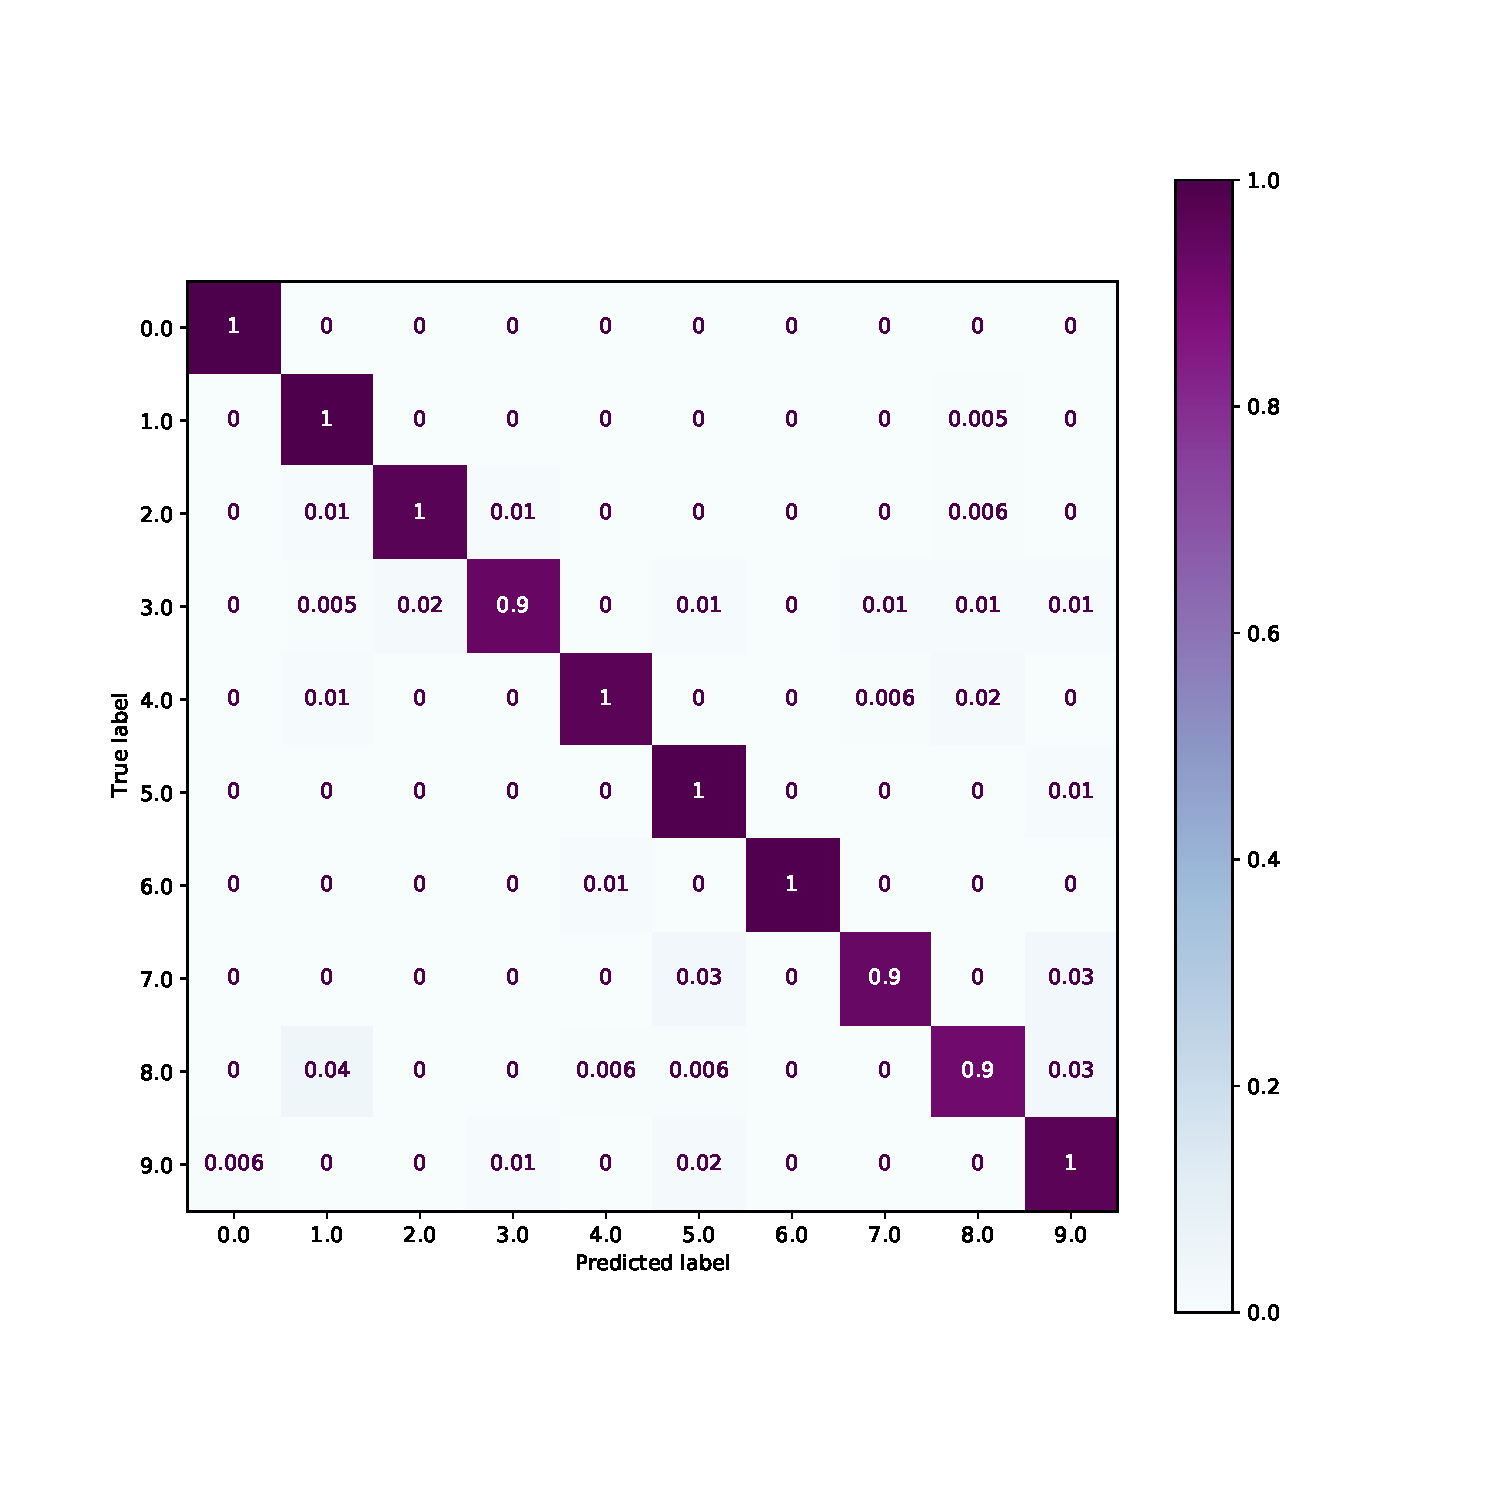
\includegraphics[width=\textwidth]{conf_mat}
    \caption{Matriz de confusión normalizada al predecir la clase de los datos de \test.}
    \label{fig:cm}
\end{figure}

Para tener una idea del error cometido con este modelo fuera de los datos trabajados, $E_{out}$ se utilizará la siguiente cota de generalización\[
E_{out}\leq E_{\test} + \sqrt{\frac{1}{2N_{\test}} \log \frac{2}{0.05}},
  \]
  esta es una cota a un nivel de confianza del 95\%.
  
  Sustituyendo el número de muestras utilizado para realizar el \test, $N_{\test} = 1797$, y el valor de $E_{\test}$, obtenemos la siguiente cota con una confianza del 95\%\[
E_{out}\leq 0.033945 + \sqrt{\frac{1}{2\cdot 1797} \log \frac{2}{0.05}} = 0.065982.
\]

Esta es una cota de generalización que nos permite hacernos una idea del comportamiento del modelo para nuevos ejemplos.

%%%%%%%%%%%%%%%%%%%%%%%%%%%%%%%%%%%%%%%%%%%%%%%%%%%%%%%%%%%%%%%%%%%%%%%%
%% 11. Suponga que Ud ha sido encargado de realizar este ajuste para una empresa. ¿Qué modelo
%% les propondría y que error E out les diría que tiene?. Justifique las decisiones.
%%%%%%%%%%%%%%%%%%%%%%%%%%%%%%%%%%%%%%%%%%%%%%%%%%%%%%%%%%%%%%%%%%%%%%%%
\subsection{Conclusiones}
%% Responder y argumentar:
%% I ¿Representa el modelo de manera adecuada los datos?
%% I ¿Consideras que la calidad del modelo es buena?
%% I ¿Es tu modelo el que proporciona el mejor error?
%% I ¿Por qué te has decidido por este modelo?
Si una empresa me encargara realizar este ajuste, propondría utilizar un modelo basado en regresión logística, para adecuarnos a la naturaleza del conjunto de datos, concretamente de la variable a predecir, una etiqueta con 10 posibles valores. Además, concretaría los hiperparámetros a utilizar, pues se han obtenido tras una validación cruzada sobre el conjunto de \training, por lo que tenemos la certeza de que se ajustan adecuadamente a los datos. Sin poder asegurar si el modelo es el que mejor se ajusta a los datos o no, podemos garantizar que, para nuevas muestras independientes, el error obtenido con este modelo es, con un 95\% de confianza, menor que 0.066, un valor que se considera lo suficientemente bajo.
\newpage

\section{\textit{Communities and Crime}}
%%% Inicio del documento

%% 1. Comprender el problema a resolver. Identificar los elementos X, Y and f del problema.
\subsection{Problema a resolver}

%% I ¿Qué base de datos tenemos?
%% I ¿Qué representan las columnas? ¿Son numéricas o
%% categóricas?
%% I ¿Qué hay en la variable de clase?
%% I ¿Se trata de un problema de aprendizaje supervisado o no
%% supervisado?
%% I ¿Es un problema de regresión o de clasificación?
Partimos de la base de datos \textit{Communities and Crime}, Comunidades y crímenes \cite{com_uci}, que trabajaremos en el archivo \texttt{ccrimes.py}.

Obtenemos cierta información consultando el archivo \texttt{communities.names}. En él se presenta esta base de datos de comunidades de Estados Unidos. Se explica que es una combinación de datos socio-económicos del censo del 1990, datos de los cuerpos policiales de la encuesta LEMAS (\textit{Law Enforcement Management and Administrative Statistics}) de 1990 y datos del UCR (\textit{Uniform Crime Reporting}) del FBI de 1995.

Es un conjunto de características multivariante, como podríamos esperar. Las características son reales y figuran escaladas en el intervalo $[0,1]$. Indican que la tarea asociada sería regresión, por tanto, nos encontramos frente a un problema de aprendizaje supervisado donde queremos predecir una variable numérica real. Hay 1994 instancias y 128 atributos, algunos de ellos con valores perdidos. Las variables fueron escogidas en función de si tenían alguna posible relación con \textit{crimen} o con la variable a predecir \textit{Per Capita Violent Crimes} (Crímenes violentos por habitante). Las variables incluidas tienen relación con la comunidad (porcentaje de la población considerado urbano, ingresos medios por familia) y con los cuerpos de seguridad (número de policías por habitante, porcentaje de policías asignados a unidades de drogas). La variable \textit{crímenes violentos por habitante} se calculó usando la población y la suma de los crímenes considerados violentos en Estados Unidos (asesinatos, violaciones, atracos y ataques). Como hubo controversia sobre si considerar la violación como crimen violento en algunas comunidades y esto originaba valores perdidos que resultaban en valores incorrectos de la variable a predecir, estas ciudades no se incluyen en el conjunto de datos (mayoritariamente del medio oeste de los Estados Unidos). Una limitación del conjunto de datos es que la encuesta LEMAS se hace en departamentos de policía con más de 100 miembros y una muestra aleatoria de departamentos más pequeños. Las comunidades que no se encontraran tanto en el censo como en las bases de datos de crímenes se omitieron, por lo que faltan muchas comunidades.

Queremos obtener información sobre el problema al que nos enfrentamos y saber de forma precisa cómo son sus variables, de qué tipos, en qué rangos se encuentran, $\cdots$ En el archivo \texttt{visualization-ccrimes.py} implementaremos el código necesario para obtener esta información. Comenzamos leyendo los nombres de los atributos y el conjunto de datos. Nuestro conjunto de datos tiene 1994 ejemplos ($N = 1994$) cada uno con 128 atributos, de los cuales 127 son numéricos (2 de ellos enteros) y 1 es una cadena de caracteres (el nombre de la comunidad). Atendiendo a la documentación, la característica \texttt{communityname} es la que se expresa como texto, además se indica que es \textit{not predictive}. El nombre de la comunidad, así como el código numérico de la misma, son únicos para cada comunidad, no aportarán información a la hora de predecir, por lo que no las utilizaremos en el proceso de aprendizaje. Buscamos las variables calificadas de \textit{not predictive} y las eliminamos del conjunto. Estas son: \texttt{state, county, community, communityname} y \texttt{fold}. Tenemos ahora un conjunto con 123 características, $n=123$.

No podemos imprimir información sobre todas las variables a la vez, ya que son demasiadas. Nos interesamos en la variable a predecir \texttt{ViolentCrimesPerPop}. Esta variable indica el número de crímenes violentos para una población de 100000 habitantes y, como el resto de variables, ha sido escalada, luego toma valores en el intervalo $[0,1]$. En la Figura \ref{fig:histVCPP} observamos su distribución. Para la mayoría de los ejemplos tiene un valor menor que 0.3.

\begin{figure}[H]
    \centering
    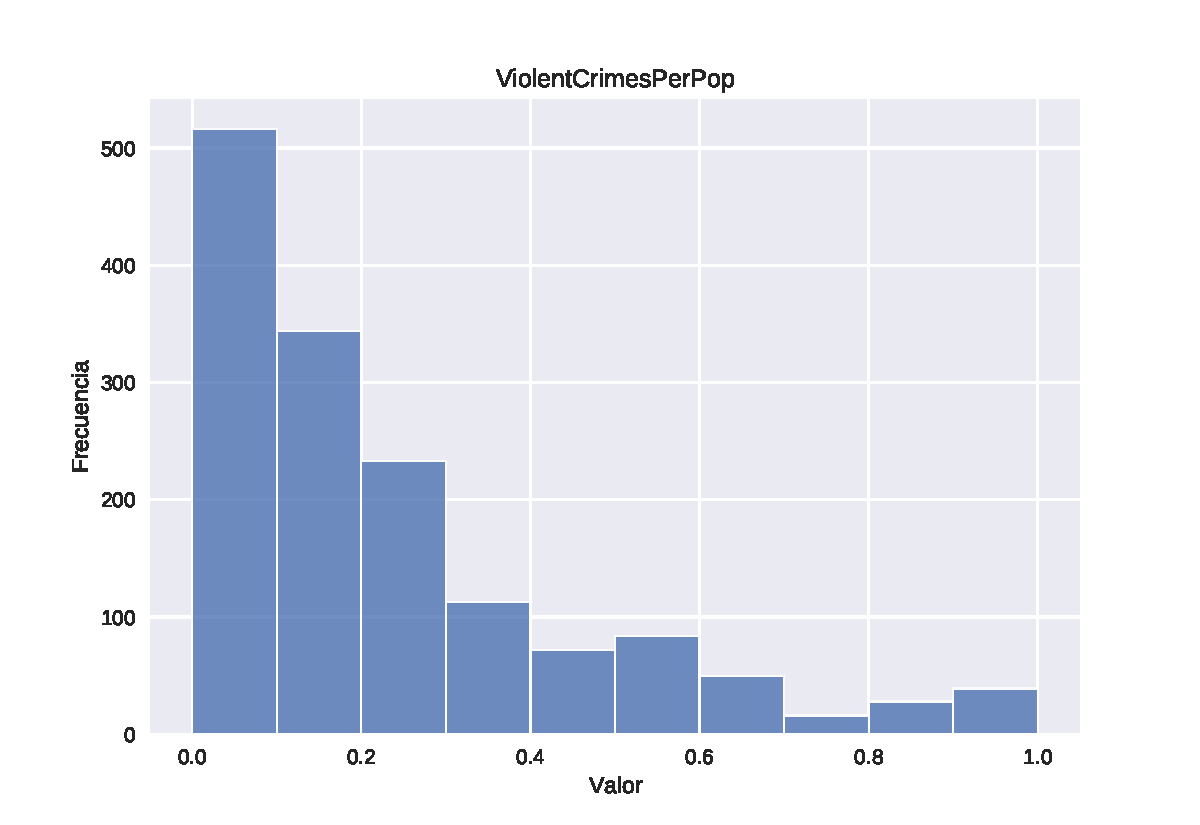
\includegraphics[width=\textwidth]{HistViolentCrimesPerPop}
    \caption{Distribución de la variable \texttt{ViolentCrimesPerPop}.}
    \label{fig:histVCPP}
\end{figure}

Continuamos obteniendo información sobre los valores perdidos, tendremos que tratar las variables que los contengan en el preprocesado y para ello debemos obtener cierta información sobre las mismas. En primer lugar, contamos el número de variables con valores perdidos: 23, que son: \texttt{OtherPerCap}, \texttt{LemasSwornFT}, \texttt{LemasSwFTPerPop}, \texttt{LemasSwFTFieldOps}, \texttt{LemasSwFTFieldPerPop}, \texttt{LemasTotalReq}, \texttt{LemasTotReqPerPop}, \texttt{PolicReqPerOffic}, \texttt{PolicPerPop}, \texttt{RacialMatchCommPol}, \texttt{PctPolicWhite}, \texttt{PctPolicBlack}, \texttt{PctPolicHisp}, \texttt{PctPolicAsian}, \texttt{PctPolicMinor}, \texttt{OfficAssgnDrugUnits}, \texttt{NumKindsDrugsSeiz}, \texttt{PolicAveOTWorked}, \texttt{PolicCars}, \texttt{PolicOperBudg}, \texttt{LemasPctPolicOnPatr}, \texttt{LemasGangUnitDeploy}, \texttt{PolicBudgPerPop}.

El porcentaje de valores perdidos en cada una de ellas es de 84.002006\%, excepto para la variable \texttt{OtherPerCap} (ingresos per capita para individuos del grupo ``otros'')  que es de 0.050150\%.

%Proseguimos el análisis de los datos estudiando las correlaciones entre las variables. Esto nos permitirá encontrar dependencias lineales entre las diferentes variables y la variable a predecir, así como relaciones lineales entre las propias variables. No todas las relaciones entre variables serán de este tipo, pero no por ello deja de ser interesante estudiar las correlaciones.

%%%%%%%%%%%%%%%%%%%%%%%%%%%%%%%%%%%%%%%%%%%%%%%%%%%%%%%%%%%%%%%%%%%%%%%%
%% 2. Selección de las clase/s de funciones a usar. Identificar cuáles y porqué.
%%%%%%%%%%%%%%%%%%%%%%%%%%%%%%%%%%%%%%%%%%%%%%%%%%%%%%%%%%%%%%%%%%%%%%%%
\subsection{Clases de funciones}
% Combinaciones lineales, cuadráticas, etc... de las observaciones.
% Justificar su uso o por qué no se consideran necesarias.
% https://scikit-learn.org/stable/modules/generated/sklearn.preprocessing.PolynomialFeatures.html#sklearn.preprocessing.PolynomialFeatures
Para realizar la predicción utilizaremos una clase de funciones lineal en el vector de pesos $w$. Como no tenemos mucha información sobre cómo se comportan los datos y qué relaciones existen entre ellos, consideramos que limitarnos a la clase \[
\mathcal{H}_0 = \{h(x) = w_0 + w_1x_1 +\cdots + w_nx_n : w \in \mathbb{R}^{n+1}\}
\]
que podría ser una primera opción natural, no será suficiente en este caso. Tenemos bastantes variables y podrían existir relaciones no lineales entre ellas. Además, combinaciones lineales de las variables podrían aportar más información que las variables por separado. Añadir complejidad a la clase de funciones nos permitirá aprovechar estas posibles relaciones no lineales entre las variables, si existieran. Es por esto, que la clase de funciones a utilizar es la de los polinomios de las variables de hasta orden 2.
 \[
\mathcal{H} = \left \{ h(x) = w_{00} +\sum_{j=1}^nw_{0j}x_j + \sum_{i,j = 1}^nw_{ij} x_ix_j: w_{kj} \in \mathbb{R} \text{ para } k = 0,\cdots, n; j=0,\cdots,n\right\}.
\]
Notamos que aunque la clase de funciones sea cuadrática en las variables $x_i$, es lineal respecto a $w$.


%%%%%%%%%%%%%%%%%%%%%%%%%%%%%%%%%%%%%%%%%%%%%%%%%%%%%%%%%%%%%%%%%%%%%%%
%% 3. Fijar conjuntos de training y test que sean coherentes.
%%%%%%%%%%%%%%%%%%%%%%%%%%%%%%%%%%%%%%%%%%%%%%%%%%%%%%%%%%%%%%%%%%%%%%
\subsection{Conjuntos de \textit{training} y \textit{test}}
%% TRAINING → Subconjunto de los datos que se estudia, se
%% visualiza y a la que se le aplican los modelos.
%% VALIDACIÓN → Subconjunto de los datos que indica cuál es el
%% mejor modelo.
%% TEST → Subconjunto de los datos que proporciona el error
%% cometido.
%% Posibles particiones:
%% I Si se decide usar el conjunto Validación: 50% training, 25%
%% Validación y 25% test.
%% I Si no se decide usar el conjunto de Validación: 70%
%% training y 30% test u 80% training y 20% test.
% https://towardsdatascience.com/train-validation-and-test-sets-72cb40cba9e7

En este caso, tenemos un único conjunto de datos. Lo dividiremos en \training y \test, puesto que utilizaremos el error cometido en el conjunto de \test para poder realizar una estimación del error fuera de la muestra. El conjunto de entrenamiento contará con un 75\% de los ejemplos y el de \test con el 25\% restante. Necesitamos más información para entrenar el modelo y calcular los hiperparámetros que para el cálculo posterior del error.

Además, para la selección del modelo utilizaremos validación cruzada con 5 particiones diferentes. Entrenaremos 5 veces los diferentes modelos, cada una de las veces entrenando con un subconjunto del 80\% de los datos de \training y usando el 20\% restante para realizar la validación. De esta manera intentamos evitar que el conjunto elegido para validación sea determinante a la hora de tomar nuestra decisión, evitando que aumente el sobreajuste.


%%%%%%%%%%%%%%%%%%%%%%%%%%%%%%%%%%%%%%%%%%%%%%%%%%%%%%%%%%%%%%%%%%%%%%%%
%% 4. Preprocesado los datos: codificación, normalización, proyección, etc. Es decir, todas las
%% manipulaciones sobre los datos iniciales hasta fijar el conjunto de vectores de caraterísticas
%% que se usarán en el entrenamiento.
%%%%%%%%%%%%%%%%%%%%%%%%%%%%%%%%%%%%%%%%%%%%%%%%%%%%%%%%%%%%%%%%%%%%%%%%
\subsection{Preprocesado}
%% ¿Por qué se preprocesan los datos?
%% Para eliminar impurezas y reducir la probabilidad de aprender de
%% manera errónea de los datos. Causas:
%% I Datos incompletos (Valores perdidos)
%% I Datos con ruido
%% I Datos inconsistentes
%% Tareas:
%% (esta lista es una sugerencia, por favor, elegid las que consideréis interesantes y/o necesarias)
%% I Colección, integración y transformación
%% Obtención de los datos, de una o más fuentes
%% Decodificación
%% Integración de datos de distintas bases de datos
%% Generación nuevo conocimiento
%% I Limpieza
%% - Modificación de datos con conflicto
%% - Eliminación de outliers
%% - Tratamiento de valores perdidos y problemas de ruido
%% I Reducción
%% - Selección de características
%% - Selección de instancias
%% - Discretización

Nos encontramos con un conjunto de 127 variables (más la variable a predecir) que ha sido previamente escalado al intervalo $[0,1]$. En primer lugar, se eliminarán las variables calificadas por los creadores de la base de datos como \textit{not predictive}. A continuación, se tratan las variables con valores perdidos, ya hemos visto que son 23.  

Para las variables que presenten valores perdidos se utilizará el siguiente criterio: si el porcentaje de valores desconocidos supera el 30\%, eliminaremos la variable, pues se considera que pasado el umbral la información que estaríamos añadiendo al problema sería demasiada y podría no coincidir con la realidad; en caso contrario, si el porcentaje de valores desconocidos es inferior al 30\%, se rellenarán estos valores mediante la técnica del vecino más cercano \cite{knnimputer}. Se barajó la opción de utilizar sustituir los valores perdidos por el valor medio para esta variable, pero esto provocaría errores grandes si nos las variables tuvieran ruido. Tras este paso, tendremos 100 de las variables originales.

Como la clase de funciones a utilizar, polinomios de las variables de hasta orden 2, añade nuevas características, pasamos de tener las 127 variables originales a tener 5151, lo que aumentará considerablemente el tiempo de cómputo. Además, como estas variables se han formado a partir de las originales, podrían, por un lado, resumir en una única variable información sobre dos de las originales, o, por otro lado, generar información redundante. Es por esto, que se procederá a seleccionar variables. Para seleccionar las variables más relevantes se utilizará la regularización LASSO, que dará un peso nulo a aquellas variables que no aporten mucha información para el proceso de aprendizaje \cite{lasso}. 

%%%%%%%%%%%%%%%%%%%%%%%%%%%%%%%%%%%%%%%%%%%%%%%%%%%%%%%%%%%%%%%%%%%%%%%%
%% 5. Fijar la métrica de error a usar. Discutir su idoneidad para el problema.
%%%%%%%%%%%%%%%%%%%%%%%%%%%%%%%%%%%%%%%%%%%%%%%%%%%%%%%%%%%%%%%%%%%%%%%%
\subsection{Métrica de error}
%% Elegir la métrica a usar y discutir su elección. Teniendo en cuenta
%% si se trata de un problema de regresión o de clasificación, así
%% como el tipo de problema a tratar.
%% I Regresión Aquí y Aquí
%% I Clasificación Aquí
Como nos encontramos ante un problema de regresión lineal, elegiremos la métrica de error usual en este tipo de problemas: error cuadrático medio. Para medir el error cometido al predecir el valor de las variables del conjunto $\{(x_1,y_1),\cdots,(x_n,y_n)\}$, donde $x_i$ es el vector de características e $y_i$ el verdadero valor de \textit{Per Capita Violent Crimes}, utilizando nuestra función hipótesis $h$, haremos:\[
E(h) = \frac{1}{n}\sum_{i=1}^n\left(y_i-h(x_i)\right)^2.
\]

%%%%%%%%%%%%%%%%%%%%%%%%%%%%%%%%%%%%%%%%%%%%%%%%%%%%%%%%%%%%%%%%%%%%%%%%
%% 8. Identificar los modelos a usar.
%%%%%%%%%%%%%%%%%%%%%%%%%%%%%%%%%%%%%%%%%%%%%%%%%%%%%%%%%%%%%%%%%%%%%%%%
\subsection{Modelos}
%% Posibles modelos a usar:
%% I Regresión lineal
%% I Regresión logística
%% I Perceptrón + Pocket
Por la naturaleza del problema, vamos a predecir una variable numérica en un intervalo, el modelo elegido es regresión lineal. No tendría sentido en este caso usar modelos como perceptrón o regresión logística, específicos para el problema de clasificación.

%%%%%%%%%%%%%%%%%%%%%%%%%%%%%%%%%%%%%%%%%%%%%%%%%%%%%%%%%%%%%%%%%%%%%%%%
%% 6. Discutir la técnica de ajuste elegida.
%%%%%%%%%%%%%%%%%%%%%%%%%%%%%%%%%%%%%%%%%%%%%%%%%%%%%%%%%%%%%%%%%%%%%%%%
\subsection{Técnica de ajuste}
%% Según modelo a usar, qué técnica de ajuste utilizas (SGD,
%% Pseudoinversa...) y razone por qué lo has elegido.

La técnica de ajuste utilizada para realizar la regresión lineal es gradiente descendente estocástico (SGD) por motivos de eficiencia. Se barajó utilizar el algoritmo de la pseudoinversa, pero se descartó por ser ineficiente. Por ello, se utilizará la función \texttt{sklearn.linear\_model.SGDRegressor}.


%%%%%%%%%%%%%%%%%%%%%%%%%%%%%%%%%%%%%%%%%%%%%%%%%%%%%%%%%%%%%%%%%%%%%%%%
%% 7. Discutir la necesidad de regularización y en su caso la justificar la función usada para ello.
%%%%%%%%%%%%%%%%%%%%%%%%%%%%%%%%%%%%%%%%%%%%%%%%%%%%%%%%%%%%%%%%%%%%%%%%
\subsection{Regularización}
%% La regularización se trata del método que penaliza la complejidad
%% del modelo, al usar función de coste. Produciendo modelos más
%% simples que generalizan mejor.
%% I L1 (Regularización Lasso) → Interesante cuando se observa
%% que algunas de las características no influyen demasiado en
%% el modelo. Al dar coeficientes a cada atributo para generar
%% la combinación de ellas, ciertos coeficientes tenderán a 0.
%% Funciona mejor cuando los atributos no están correlados
%% entre sí.
%% I L2 (Regularización Ridge) → Útil cuando parezca que
%% varios de los atributos están correlados entre ellos.
%% Hace que los coeficientes sean pequeños.
%% Funciona mejor cuando la mayoría de los atributos son
%% relevantes.
Tenemos muchas variables y no todas podrían ser igual de relevantes. Por un lado, se ha utilizado regularización LASSO como método para selección de variables, pues antes de esto algunas de las variables podrían no aportar información nueva y este método haría que sus coeficientes fuesen 0, permitiéndonos descartarlas.

Por otro lado, se ha utilizado una técnica de regularización para evitar el sobreajuste a la hora de ajustar el modelo. Con ello, disminuiremos la complejidad del modelo y haremos decrecer el término del error proveniente de la varianza.

Se utilizará regularización Ridge, que, a diferencia de LASSO, no pone coeficientes a 0 con frecuencia. Penaliza a aquellos coeficientes que sean muy grandes, así, al realizar el ajuste, el peso de una variable no influirá mucho más que el resto. De esta forma, disminuiremos la complejidad del modelo sin dejar de usar ninguna variable. El modelo a usar, \texttt{sklearn.linear\_model.SGDRegressor}, utiliza por defecto este tipo de regularización, luego no será necesario indicarlo de manera adicional.


%%%%%%%%%%%%%%%%%%%%%%%%%%%%%%%%%%%%%%%%%%%%%%%%%%%%%%%%%%%%%%%%%%%%%%%%
%% 9. Estimación de hiperparámetros y selección del mejor modelo.
%%%%%%%%%%%%%%%%%%%%%%%%%%%%%%%%%%%%%%%%%%%%%%%%%%%%%%%%%%%%%%%%%%%%%%%%
\subsection{Estimación de hiperparámetros y selección del mejor modelo}\label{sec:hp}
%% 1. Ajustar los hiperparámetros del modelo.
%% 2. Ajustar los datos de validación (o test).
%% 3. Seleccionar el que se considera el mejor de los modelos y
%% argumentar por qué se elige.
Se han considerado tres tipos de parámetros a ajustar en este modelo. Por un lado, el valor de \texttt{alpha}, la constante de regularización, para la que se probaron los valores: 0.1, 0.01, 0.001 y 0.0001. Para la tasa de aprendizaje, \texttt{learning\_rate}, se consideraron las diferentes opciones ofrecidas por la biblioteca: \texttt{'constant', 'optimal','invscaling', 'adaptive'}. Por último, se prueban diferentes valores para el número máximo de iteraciones: 5000, 10000 y 15000.

Para seleccionar el mejor modelo se probarán las diferentes combinaciones de los parámetros en el conjunto de entrenamiento mediante validación cruzada. Este proceso se implementa con ayuda de la función \texttt{sklearn.model\_selection.GridSearchCV}. Hay que tener en cuenta que esta función maximiza el parámetro \texttt{scoring}, por lo que, para obtener el modelo con menor error cuadrático medio, calculamos su negación. En la Tabla \ref{tab:r} se recogen los errores obtenidos con los diferentes parámetros (el error ya positivo), se eliminan los resultados obtenidos con \texttt{learning\_rate = 'optimal'} por ser considerablemente superiores a los demás.

\begin{table}[H]
\large
\centering
\caption{Error cuadrático medio obtenido con los diferentes hiperparámetros.}
\label{tab:r}
\begin{tabular}{lrrr}
\toprule
Error cuadrático medio & \texttt{alpha} & \texttt{learning\_rate} & \texttt{max\_iter}\\ \midrule
0.019 & 0.1 & \texttt{constant} & 5000\\
0.019 & 0.1 & \texttt{constant} & 10000\\
0.019 & 0.1 & \texttt{constant} & 15000\\
0.019 & 0.1 & \texttt{invscaling} & 5000\\
0.019 & 0.1 & \texttt{invscaling} & 10000\\
0.019 & 0.1 & \texttt{invscaling} & 15000\\
0.018 & 0.1 & \texttt{adaptive} & 5000\\
0.018 & 0.1 & \texttt{adaptive} & 10000\\
0.018 & 0.1 & \texttt{adaptive} & 15000\\\\[-10pt]
0.016 & 0.01 &\texttt{constant} & 5000\\
0.015 & 0.01 &\texttt{constant} & 10000\\
0.015 & 0.01 &\texttt{constant} & 15000\\
0.017 & 0.01 &\texttt{invscaling} & 5000\\
0.017 & 0.01 &\texttt{invscaling} & 10000\\
0.017 & 0.01 &\texttt{invscaling} & 15000\\
0.015 & 0.01 &\texttt{adaptive} & 5000\\
0.015 & 0.01 &\texttt{adaptive} & 10000\\
0.015 & 0.01 &\texttt{adaptive} & 15000\\\\[-10pt]
0.015 & 0.001 &\texttt{constant} & 5000\\
0.015 & 0.001 &\texttt{constant} & 10000\\
0.015 & 0.001 &\texttt{constant} & 15000\\
0.017 & 0.001 &\texttt{invscaling} & 5000\\
0.017 & 0.001 &\texttt{invscaling} & 10000\\
0.017 & 0.001 &\texttt{invscaling} & 15000\\
0.014 & 0.001 &\texttt{adaptive} & 5000\\
0.014 & 0.001 &\texttt{adaptive} & 10000\\
0.014 & 0.001 &\texttt{adaptive} & 15000\\\\[-10pt]
0.015 & 0.0001 &\texttt{constant} & 5000\\
0.015 & 0.0001 &\texttt{constant} & 10000\\
0.015 & 0.0001 &\texttt{constant} & 15000\\
0.017 & 0.0001 &\texttt{invscaling} & 5000\\
0.017 & 0.0001 &\texttt{invscaling} & 10000\\
0.017 & 0.0001 &\texttt{invscaling} & 15000\\
0.014 & 0.0001 &\texttt{adaptive} & 5000\\
0.014 & 0.0001 &\texttt{adaptive} & 10000\\
0.014 & 0.0001 &\texttt{adaptive} & 15000\\
\bottomrule
\end{tabular}
\end{table}

Tras la ejecución de la validación cruzada, elegimos como mejor modelo aquel que obtiene menor error cuadrático medio en la media de las validaciones. Este es regresión lineal tomando \texttt{alpha = 0.0001}, \texttt{learning\_rate = 'adaptive'}, \texttt{max\_iter = 10000}.

%%%%%%%%%%%%%%%%%%%%%%%%%%%%%%%%%%%%%%%%%%%%%%%%%%%%%%%%%%%%%%%%%%%%%%%%
%% 10. Estimación por validación cruzada del error E out del modelo. Compárela con E test , ¿que
%% conclusiones obtiene?
%%%%%%%%%%%%%%%%%%%%%%%%%%%%%%%%%%%%%%%%%%%%%%%%%%%%%%%%%%%%%%%%%%%%%%%%
\subsection{Estimación del error}
%% Especificar el error que se produce al ajustar el modelo.
En la validación cruzada se obtiene el siguiente error\[
E_{\text{CV}} = 0.014431164996118306.\]

Al usar el modelo para predecir la variable objetivo con los datos de \test y compararlo con el valor real se obtiene el error\[
E_{\test} = 0.0233.
\]

El error cometido en los datos de \test es mayor que el error de la validación cruzada. Pero es el error en \test el que nos dará una cota más precisa del error fuera de la muestra, $E_{\textit{out}}$. En este caso, no podremos utilizar las cotas de generalización estudiadas en clase, específicas del problema de clasificación (pues utilizaban su error). Es por ello, que la estimación más precisa que tenemos del error fuera de la muestra es el $E_{\test}$, ya que son unos datos independientes del conjunto utilizado para ajustar el modelo. Diremos que el error fuera de la muestra será aproximadamente 0.0233, pero no tenemos, como en el caso anterior, un nivel de confianza establecido para esa afirmación.

Es normal que el error fuera de la muestra, en puntos no utilizados para entrenar sea mayor que el error en los datos utilizados para entrenar. La estimación obtenida con la validación cruzada sería una cota muy optimista del error.

%%%%%%%%%%%%%%%%%%%%%%%%%%%%%%%%%%%%%%%%%%%%%%%%%%%%%%%%%%%%%%%%%%%%%%%%
%% 11. Suponga que Ud ha sido encargado de realizar este ajuste para una empresa. ¿Qué modelo
%% les propondría y que error E out les diría que tiene?. Justifique las decisiones.
%%%%%%%%%%%%%%%%%%%%%%%%%%%%%%%%%%%%%%%%%%%%%%%%%%%%%%%%%%%%%%%%%%%%%%%%
\subsection{Conclusiones}
%% Responder y argumentar:
%% I ¿Representa el modelo de manera adecuada los datos?
%% I ¿Consideras que la calidad del modelo es buena?
%% I ¿Es tu modelo el que proporciona el mejor error?
%% I ¿Por qué te has decidido por este modelo?
Para realizar un ajuste de la base de datos dada, atendiendo a la naturaleza del problema y el tipo de variable a predecir, propondría utilizar regresión lineal con los hiperparámetros seleccionados en la Sección \ref{sec:hp}.\\

Consideramos que la calidad del modelo es buena, ha sido el que ha obtenido menor error en validación cruzada entre las diferentes opciones tenidas en cuenta. Además, podemos asegurar, asumiendo que las muestras con las hemos trabajado son independientes y tienen una distribución común que no cambiará, que el error fuera de la muestra es menor o igual que 0.0233. Cuando traten de predecir el número de crímenes violentos por habitante en nuevas comunidades a partir de la información necesaria, podrán tener confianza en que el error obtenido en la predicción es menor que este valor.
\newpage

%%%%%%%%%%%%%%%%%%%%%%%%%%%%
\printbibliography
% https://realpython.com/pandas-python-explore-dataset/
\end{document}
